\documentclass[aps,prx,twocolumn,10pt,superscriptaddress,nofootinbib,longbibliography,floatfix]{revtex4-2}

\usepackage{amsmath,amssymb,amsfonts}
\usepackage{bm}
\usepackage{graphicx}
\usepackage{booktabs}
\usepackage{xcolor}
\usepackage{hyperref}
\graphicspath{{figures/}}
\hypersetup{colorlinks=true,linkcolor=blue,citecolor=blue,urlcolor=blue}

\newcommand{\dd}{\mathrm{d}}
\newcommand{\aexc}{\alpha_{\rm exc}}
\newcommand{\Ham}{\mathcal{H}}
\newcommand{\Mom}{\mathcal{M}}
\newcommand{\Egeo}{\mathcal{E}_{\rm geo}}
\newcommand{\KC}{K_{\rm C}}
\newcommand{\Et}{\tilde{E}}
\newcommand{\Bt}{\tilde{B}}
\newcommand{\Nppc}{N_{\rm ppc}}
\newcommand{\lcap}{\ell_{\rm cap}}
\newcommand{\rbar}{\bar{r}}

\renewcommand{\topfraction}{0.9}
\renewcommand{\dbltopfraction}{0.9}
\renewcommand{\textfraction}{0.07}
\renewcommand{\floatpagefraction}{0.75}
\renewcommand{\dblfloatpagefraction}{0.75}

\begin{document}

\IfFileExists{sections/title.tex}{\title{Hybrid symplectic-cubature and moving-finite-volume solver\texorpdfstring{\\}{ } for general-relativistic kinetic matter}

\author{Author list to be set}
\noaffiliation

\date{\today}

\begin{abstract}
Kinetic matter in strong gravitational fields spans two disparate regimes that challenge any single discretization: collisionless phase-space streaming with sharp orbital caustics and collisional relativistic plasma near local thermodynamic equilibrium. Meshless moving-finite-volume moment closures remove sampling noise across finite mean free paths, whereas fourth-order symplectic packet integration preserves geodesic invariants in curved spacetimes without neighbor diffusion. We combine both approaches in a unified GPU-accelerated general-relativistic solver built atop AthenaK. For collisional flows, an asymptotic-preserving finite-volume scheme evolves covariant velocity bases under boosted one-sided Riemann integrals blended continuously into a Synge HLLC fluid solver, alongside a conservative relativistic Cell-BGK packet collision operator driven by a globally dominating Gamma-mixture Maxwell-J{\"u}ttner sampler and exact convex four-momentum projection. This operator enforces energy conservation to rounding precision across four decades of optical depth at constant step cost, achieving a fiftyfold speedup over subcycled Monte Carlo binary pairing in optically thick shocks. For collisionless strong-field transport, deterministic Stroud cubature, spherical Lebedev shells, and symmetry-exact quasi-Monte Carlo sampling pair with a fourth-order two-stage Gauss-Legendre symplectic pusher, three-level quadratic Lagrange metric time interpolation, zero-VRAM-overhead $C^2$ quintic Hermite spatial reconstruction, stage-accurate causal Z4c coupling, multi-rate subcycling, and a self-adjoint harmonic flux-conservative deposit filter (directional or unsplit seven-point with active-block skipping). Across $6$-level Kerr clusters, $C^2$ quintic reconstruction breaks the $\mathcal{O}(\Delta x^3)$ spatial error floor by $311\times$ down to $|\Delta\Egeo/\Egeo|_{\rm med} = 3.38 \times 10^{-10}$, while high-Courant \texttt{rk3} integration, active-block unsplit filtering, and multi-rate subcycling accelerate single-GPU simulations by $3.19\times$ in Kerr SMR and $2.24\text{--}2.95\times$ in $3+1$ dynamical collapse. Benchmarks from relativistic colliding beams and hundred-thousand-particle Kerr tidal flows through dynamical black hole mergers, prolate spindle collapse, Shapiro-Teukolsky star clusters spanning equilibrium, migration, collapse, and dispersal, and self-gravitating Jeans binary black hole formation establish unified accuracy and strong scaling on a single graphics accelerator.
\end{abstract}

\maketitle
}{}

\IfFileExists{sections/introduction.tex}{\section{Introduction}\label{sec:intro}

Self-gravitating and horizon-crossing relativistic kinetic matter underlies a wide class of strong-field astrophysical systems, from relativistic star clusters and dark-matter spikes around spinning black holes to stellar tidal debris, extreme-mass-ratio back-reaction, and marginally collisional neutrino transport in core collapse and compact-binary mergers~\cite{1985ApJ...298...34S,1985ApJ...298...58S,Shapiro:1991zza,Andreasson:2011ng,Acuna-Cardenas:2021nkj}. Across these environments, the ratio of mean free path to macroscopic dynamical scale varies by many orders of magnitude. Dilute clusters and photon rays stream freely along geodesics with vanishing scattering, whereas dense shocked layers relax swiftly toward local relativistic Maxwell--J\"uttner equilibrium. Modeling both regimes consistently inside a dynamical three-plus-one spacetime poses coupled challenges in symplectic orbit integration, spatial metric regularity, discrete stress-energy conservation across adaptive meshes, causal spacetime source coupling, and asymptotic collisional stiffness.

Two distinct numerical paradigms address kinetic transport in curved spacetime. Particle-in-cell methods represent the phase-space distribution as an ensemble of finite-mass macroparticles pushed along geodesics and deposited onto an Eulerian curvature mesh~\cite{Shibata:1999va,Shibata:1999wi,East:2019bwu,Galishnikova:2025pfi,Wu:2026nrpic}. The baseline numerical-relativity particle-in-cell (NRPIC) formulation~\cite{Wu:2026nrpic} demonstrated full three-dimensional Einstein--Vlasov evolutions in AthenaK~\cite{2026ApJS..283...27S,Zhu:2024utz} using second-order implicit midpoint and spacetime Boris pushers, four-point cubic Hermite metric interpolation, cloud-in-cell adaptive deposition, and plain binomial filtering. Conversely, meshless moving-finite-volume (MFM) closures~\cite{Hopkins:2015mfc,Hopkins:2026lbv} expand velocity space locally into Gaussian or top-hat basis elements coupled through boosted one-sided Riemann fluxes, eliminating finite-sample Poisson noise in collisional and marginally kinetic flows.

Four concrete numerical barriers limit existing particle-mesh and kinetic-relativity algorithms when pushed to extreme strong-field accuracy, self-gravitating longevity, or optical-depth transitions. First, second-order trajectory pushers accumulate secular orbital phase lag during strong-field zoom-whirl and light-ring passages, while tetrad-projected Boris updates inherit gauge-dependent truncation errors from local spatial triads~\cite{Olivares:2021cfa,Boyeneni:2025tsx,Wu:2026nrpic}. Even when temporal integration reaches machine precision, standard four-point cubic Hermite reconstruction leaves cell-face gradient discontinuities of third order in grid spacing that impose an irreducible spatial error floor on static-mesh invariants. Second, plain binomial deposit filters act uniformly in coordinate space and leak proper-volume energy whenever the spatial metric determinant varies steeply or when clouds straddle adaptive refinement jumps, whereas pre-densitized filters distort constant curved states~\cite{1991ppcs.book.....B,Wu:2026nrpic}. Third, holding deposited sources frozen across Runge--Kutta spacetime stages injects a first-order temporal coupling bias that restricts stable Courant numbers and locks particle pushes to every mesh step. Fourth, binary Monte Carlo pairing scales linearly with optical depth and stalls in dense shocks, whereas continuum velocity bases incur diffusive broadening across curved multi-stream caustics.

Here we derive, prove discrete invariants for, and benchmark a unified formulation inside AthenaK that removes all four barriers simultaneously. For geodesic transport of both massive macroparticles and null rays, a canonical two-stage fourth-order Gauss--Legendre implicit Runge--Kutta (GL4) pusher~\cite{SanzSerna:1988} operates directly in Darboux phase-space coordinates alongside three-level quadratic metric time interpolation and a zero-overhead twice-continuously-differentiable ($C^2$) six-node quintic Hermite spatial reconstruction fitting inside the standard four-ghost-cell stencil. For mesh feedback, a self-adjoint metric-weighted flux-conservative filter built around harmonic face conductances preserves constant states, machine-precision proper-volume integrals across arbitrary adaptive boundaries, $L^2$ contractivity, and unconditional pointwise positivity in both directional sweeps and an unsplit seven-point active-block stencil with boundary-only reflux storage. Causal stage-accurate source reconstruction removes first-order frozen-matter errors and allows stable three-stage strong-stability-preserving Runge--Kutta (SSP-RK3) spacetime steps at high Courant factors together with continuous multi-rate matter subcycling and a puncture-split elliptic constraint solver for self-gravitating black hole initial data~\cite{Bowen:1980yu}. Across finite mean free paths, Lagrangian velocity bases blend continuously from boosted kinetic fluxes into a Synge relativistic hydrodynamic Riemann solver~\cite{Synge:1957,Mignone:2005ns}, while a packet Cell-BGK relaxation operator sampled via a globally dominating Gamma-mixture Maxwell--J\"uttner envelope and exact convex four-momentum projection spans collisionless free streaming through thick shocks at constant cost per step~\cite{Israel:1963,Anderson:1974}. Symmetry-exact quasi-Monte Carlo pairing~\cite{Sobol:1967} and deterministic Stroud and Lebedev cubature rules~\cite{Stroud:1971,Lebedev:1976} eliminate net linear momentum drift and suppress artificial remnant black hole spin in self-gravitating collapse.

Five core findings emerge across flat-space, stationary Kerr, and full three-plus-one dynamical benchmarks. (i) Replacing global iterative root searches and neighbor-grid degeneracies with safeguarded analytical Newton solves and compact kernel layouts cuts collisional finite-volume runtime substantially while keeping finite-volume parity. (ii) Conservative Cell-BGK packet relaxation matches exact collisionless characteristics and relativistic Taub shocks across four decades of cross section while outperforming subcycled Monte Carlo collisions by more than an order of magnitude in throughput. (iii) Canonical GL4 integration combined with $C^2$ quintic Hermite metric reconstruction reduces eccentric near-extremal Kerr energy drift by six orders of magnitude, eliminates the cubic-Hermite spatial floor by more than two orders of magnitude without auxiliary spline arrays, and resolves near-critical photon-sphere separatrices accurately. (iv) Self-adjoint harmonic conservative filtering eliminates percent-to-tens-of-percent curved-metric deposit leakage down to rounding precision, and its unsplit active-block formulation reduces communication three-fold while delivering multi-fold static-mesh acceleration. (v) Causal stage-accurate source coupling restores clean temporal convergence in gravitational collapse, supports high-Courant SSP-RK3 evolution with multi-rate subcycling across Oppenheimer--Snyder, Shapiro--Teukolsky, binary cluster, and massive-particle black hole back-reaction tests, and pairs with symmetry-exact sampling to hold net linear momentum below fourteen orders of magnitude while preventing spurious orbital recoil and spin contamination.

We organize the presentation into system equations, algorithmic derivations and invariant proofs, validation across special-relativistic and Kerr testbeds, and full dynamical three-plus-one benchmarks. Section~\ref{sec:system} states the unified 3+1 ADM and Z4c spacetime system, Darboux kinetic equations, and Synge closures. Section~\ref{sec:method} develops each stage of the high-order, metric-conservative, and collisional algorithm with proofs of symplecticity, $C^2$ regularity, discrete conservation, and sampling domination. Section~\ref{sec:sr_regimes} verifies flat-space convergence and optical-depth shock transitions; Sec.~\ref{sec:kerr} benchmarks Kerr shear flows, extreme zoom-whirl and light-ring geodesics, and static-mesh clusters; Sec.~\ref{sec:collapse} validates dynamical collapse, massive-particle black hole back-reaction, and end-to-end comparisons against baseline second-order NRPIC; and Sec.~\ref{sec:conclusions} summarizes our findings. Detailed initial-data prescriptions and benchmark ledgers appear in Appendices~\ref{app:sampling} and~\ref{app:params}, and complete metric, constraint, and device profiling tables appear in the Supplemental Material.
}{}
\IfFileExists{sections/system.tex}{\section{Relativistic kinetic system in 3+1 form}\label{sec:system}

Consider massive particles of rest mass $\mu_p$ moving along timelike trajectories on the future mass shell $g^{\mu\nu} u_\mu u_\nu = -1$, where $u_\mu$ denotes covariant four-velocity per unit rest mass. Under a three-plus-one Arnowitt-Deser-Misner foliation \cite{Arnowitt:1962hi} of slices $\Sigma_t$ with lapse $\alpha$, shift $\beta^i$, induced spatial metric $\gamma_{ij}$, inverse $\gamma^{ij}$, and determinant $\gamma = \det(\gamma_{ij})$, the spacetime line element is
\begin{equation}
\dd s^2 = -\alpha^2\,\dd t^2 + \gamma_{ij}(\dd x^i + \beta^i\,\dd t)(\dd x^j + \beta^j\,\dd t).
\end{equation}
Normal observers pierce $\Sigma_t$ orthogonally along $n_\mu = (-\alpha,0,0,0)$ and $n^\mu = (\alpha^{-1}, -\alpha^{-1}\beta^i)$, measuring the Lorentz factor
\begin{equation}
W = -n^\mu u_\mu = \sqrt{1 + \gamma^{ij} u_i u_j},
\end{equation}
and the raised spatial components $u^i = \gamma^{ij} u_j$. The single-particle Hamiltonian in canonical Darboux coordinates $(x^i, u_i)$ equals the coordinate energy $-u_0 = \alpha W - \beta^i u_i$. Hamilton's equations therefore give the normal-observer characteristic equations,
\begin{align}\label{eq:characteristics}
\frac{\dd x^i}{\dd t} &= \frac{\alpha \gamma^{ij} u_j}{W} - \beta^i, \nonumber\\
\frac{\dd u_i}{\dd t} &= -W \partial_i \alpha + u_j \partial_i \beta^j + \frac{\alpha}{2W} u^l u^m \partial_i \gamma_{lm}.
\end{align}

On the mass shell the Lorentz-invariant momentum volume element is $\dd\Pi_u = \dd^3 u / (\sqrt{\gamma}\,W)$, while the proper spatial volume on $\Sigma_t$ is $\sqrt{\gamma}\,\dd^3 x$. Their product equals the flat coordinate measure $\dd^3 x\,\dd^3 u$. Defining the Darboux rest-mass phase-space density $f(t, \bm{x}, \bm{u}) \equiv \sqrt{\gamma}\,W\,\mathcal{F}$ from the scalar distribution function $\mathcal{F}$ absorbs every geometric volume factor. Because the normal-observer characteristic equations are Hamiltonian, their phase-space divergence vanishes identically, yielding the Darboux Vlasov law
\begin{equation}\label{eq:darboux_vlasov}
\frac{\partial f}{\partial t} + \frac{\partial}{\partial x^i}\!\left(\frac{\dd x^i}{\dd t} f\right) + \frac{\partial}{\partial u_i}\!\left(\frac{\dd u_i}{\dd t} f\right) = \left(\frac{\partial f}{\partial t}\right)_{\rm coll}.
\end{equation}
Unconstrained covariant momenta $\bm{u} \in \mathbb{R}^3$ keep particle three-velocities strictly subluminal without artificial velocity-space barriers, and coordinate derivatives vanish globally when the slice is flat Minkowski space.

Normal observers project the stress-energy tensor $T^{\mu\nu}$ into coordinate-densitized energy, momentum, and spatial stress fields via moments of $f$:
\begin{equation}\label{eq:adm_sources}
\sqrt{\gamma}\begin{pmatrix} E \\ S_i \\ S_{ij} \end{pmatrix} = \int_{\mathbb{R}^3} \begin{pmatrix} W \\ u_i \\ u_i u_j / W \end{pmatrix} f(t,\bm{x},\bm{u})\,\dd^3 u.
\end{equation}
Dividing these integrals by $\sqrt{\gamma}$ supplies the matter sources to Einstein's equations evolved in the constraint-damped Z4c formulation \cite{Bona:2003fj,Hilditch:2012fp,Gundlach:2005eh} under moving-puncture gauge \cite{Bona:1994dr,Campanelli:2005dd,Alcubierre:2002kk}.

When interparticle scattering with reduced cross section $\sigma/\mu_p$ is active, local relaxation drives $\mathcal{F}$ toward the relativistic Maxwell-J{\"u}ttner equilibrium at dimensionless temperature $\theta \equiv k_B T / \mu_p$, characterized by specific enthalpy $h_{\rm rel}(\theta) = K_3(1/\theta)/K_2(1/\theta)$ and mean Lorentz factor $\bar{W}_{\rm com}(\theta) = h_{\rm rel}(\theta) - \theta$ in the Synge gas equation of state \cite{Synge:1957,Israel:1963}. In the collisionless limit $\sigma/\mu_p = 0$, the Darboux Vlasov law reduces to exact phase-space conservation along geodesics.

}{}
\IfFileExists{sections/method.tex}{\section{Hybrid phase-space algorithm}\label{sec:method}

The physical demands of strong-field kinetic flows split along collisionality. Where $\sigma/\mu_p > 0$, thermalization smooths velocity-space filamentation and hydrodynamic shocks emerge; moving-finite-volume velocity moments with an asymptotic Riemann blend avoid Monte Carlo noise and enforce conservation across all optical depths. Where $\sigma/\mu_p = 0$, caustic crossing and tidal stretching amplify neighbor-diffusion errors in moment closures; evolving deterministic cubature packets along characteristics eliminates spatial smearing and conserves invariants to integration tolerance.

\subsection{Moving-finite-volume basis discretization}\label{sec:method_mfm}

On $N$ moving mesh-generating elements at positions $\bm{x}_a(t)$, the cubic spline kernel $W(\bm{r}, h_a)$ defines the partition volume $V_a = \bar{n}_a^{-1}$ through $h_a^3 \bar{n}_a = 1$, alongside the coordinate kernel moment matrix $\bm{E}_a = \sum_c (\bm{x}_{ca}\otimes\bm{x}_{ca}) W(\bm{x}_{ca}, h_a)$ and antisymmetric effective face area covectors $A_{ab,i} = V_a(\bm{E}_a^{-1}\bm{x}_{ba})_i W(\bm{x}_{ba},h_a) + V_b(\bm{E}_b^{-1}\bm{x}_{ba})_i W(\bm{x}_{ba},h_b)$ \cite{Hopkins:2015mfc,Hopkins:2026lbv}. Regularizing $\bm{E}_a$ when one-sided vacuum stencils become ill-conditioned preserves exact face antisymmetry $A_{ab,i} = -A_{ba,i}$.

Within each element $a$, the momentum distribution is expanded in $N_b$ moving velocity bases with compact top-hat or Gaussian support, evolving conserved moments $(m_{a,\alpha}, P_{a,\alpha,i}, \Pi_{a,\alpha,ij})$ that recover rest-mass density $D_{a,\alpha} = m_{a,\alpha}/V_a$, mean covariant velocity $\bar{u}_{a,\alpha,i}$, and symmetric covariance $\Sigma_{a,\alpha,ij} = \Pi_{a,\alpha,ij}/m_{a,\alpha} - \bar{u}_{a,\alpha,i}\bar{u}_{a,\alpha,j}$. Sylvester minor checks verify positive-definiteness during gradient limiting and realizability repair, calling full eigendecomposition only for borderline degenerate tensors. At each cell interface, Cholesky orthogonalization transforms the reconstructed basis moments into a normal-observer face triad $(\hat{e}_{(1)}^i, \hat{e}_{(2)}^i, \hat{e}_{(3)}^i)$. On each transverse quadrature slice $\bm{u}_\perp$, the parallel flux integral reduces to the sliced flux antiderivatives for moments of $(u_{(1)}/W - \beta_F)$ with exact Gauss-Legendre switchover in cold regimes \cite{Hopkins:2026lbv}. Demanding zero net rest-mass exchange gives the zero-mass-flux root condition $\Phi(\beta_F) = 0$ for the normal-observer face speed $\beta_F \in (-1,1)$, solved via safeguarded analytical Newton iterations using the exact derivative $\partial\Phi/\partial\beta_F$. Pairs of bases across each face match in the Lorentz-boosted face rest frame when $|\beta_F| < 1$, and element centers advance at the mass-weighted coordinate drift velocity inside a two-stage second-order Runge-Kutta Strang step.

\subsection{Symplectic cubature packets for collisionless matter}\label{sec:method_scp}

When $\sigma/\mu_p \le 0$, warm moment closures suffer artificial dispersion from spatial gradient limiting and basis-pair mixing. Instead, the solver initializes deterministic phase-space packets directly from each populated velocity basis $(a,\alpha)$ using fifth-degree symmetric Stroud cubature in three dimensions \cite{Stroud:1971}:
\begin{equation}\label{eq:scp_map}
\bm{u}_{a,\alpha,q} = \bar{\bm{u}}_{a,\alpha} + \bm{L}_{a,\alpha}\bm{R}_{a,\alpha}\bm{\xi}_q, \qquad m_{a,\alpha,q} = m_{a,\alpha} w_q,
\end{equation}
where $\bm{L}_{a,\alpha}\bm{L}_{a,\alpha}^T = \Sigma_{a,\alpha}$ is the Cholesky factor and $(\bm{\xi}_q, w_q)$ are positive-weight unit-covariance nodes scaled to match the uniform top-hat cube or Gaussian normal moments up to fifth order ($Q_{\rm SCP} = 14$ nodes by default, $8$ or $27$ optional, collapsing to $1$ cold packet when $\mathrm{Tr}\,\Sigma_{a,\alpha}$ vanishes). Every populated element receives an independent orthogonal frame $\bm{R}_{a,\alpha} \in \mathrm{SO}(3)$ generated via Shoemake's uniform quaternion parameterization from the base-$2,3,5$ Halton low-discrepancy sequence \cite{Halton:1960}. Because $\bm{R}_{a,\alpha}$ preserves orthogonality, the cubature packet expansion matches zeroth, first, and second velocity moments identically while suppressing lattice-aligned velocity-space resonances along curved orbits. Packets subsequently evolve by fixed-point implicit midpoint integration of the normal-observer characteristic equations without neighbor searches, inter-element fluxes, or gradient diffusion, depositing stress-energy onto the adaptive mesh via cloud-in-cell or higher-order B-spline clouds \cite{Wu:2026nrpic}.

\subsection{Collisional relaxation and asymptotic HLLC blend}\label{sec:method_ap}

In collisional runs, local cell energy $\mathcal{E}_a$ and momentum $P_{a,i}$ are boosted into the center-of-momentum frame to extract the invariant specific energy $\bar{W}_{\rm com}$. A combined asymptotic-Chebyshev evaluation of $K_2$ and $K_3$ paired with analytical Newton inversion solves $\bar{W}_{\rm com}(\theta) = K_3(1/\theta)/K_2(1/\theta) - \theta$ for the kinetic temperature $\theta$ and adiabatic index $\Gamma_{\rm ad} \in [4/3, 5/3]$ \cite{Synge:1957}. The hard-sphere Maxwell-J{\"u}ttner collision rate $\nu_a = n_a(\sigma/\mu_p)\mathcal{R}_{\rm MJ}(\theta)$ drives convex intra-cell BGK relaxation \cite{Anderson:1974,Israel:1963}, locked to exact total momentum and energy by a one-dimensional scalar dispersion adjustment. Across element faces, the kinetic one-sided flux is blended continuously with a relativistic Synge-equation-of-state HLLC fluid Riemann solver \cite{Mignone:2005ns} and Noh thermal conduction \cite{Noh:1987} using the asymptotic face blend factor $w_c = \exp(-\Delta x_{\rm prop} D_f \sigma / (\mu_p \sqrt{\gamma_f}))$, guaranteeing second-order consistency from free streaming ($w_c = 1$) to dense relativistic hydrodynamics ($w_c \to 0$).

\subsection{GPU hash scaling and kernel layout}\label{sec:method_gpu}

Achieving high GPU throughput in the MFM branch requires eliminating two bottlenecks. First, strong shear broadens the smoothing-length ratio $h_{\max}/h_{\min}$ at cluster edges; sizing the spatial hash cell width by the mean smoothing length $\bar{h}$ while using per-element search stencils and symmetric gather-scatter neighbor construction prevents quadratic search collapse while yielding identical sorted neighbor lists. Second, Kokkos kernels capturing views above five hundred bytes spill parameters to device constant memory and inject host event synchronizations on every launch. Packing device array pointers into compact plain-old-data structures and specializing flat Minkowski and analytic Kerr metric evaluations keeps all continuum flux, gradient, and relaxation kernels in fast local launch paths without altering physical equations.
}{}
\IfFileExists{sections/results_regimes.tex}{\section{Special-relativistic convergence and optical-depth transition}\label{sec:sr_regimes}

We first verify spatial convergence order, relativistic multi-stream pairing, and asymptotic collisional crossover on flat three-dimensional periodic domains in normal-observer Cartesian coordinates ($\alpha = 1$, $\beta^i = 0$, $\gamma_{ij} = \delta_{ij}$).

Warm sound-like perturbations test continuum spatial convergence cleanly away from shock discontinuities. Initializing a single relativistic top-hat velocity basis with mean boost $\bar{u}_x = 0.3$, uniform density modulation amplitude $0.05$, and isotropic momentum dispersion $\sigma_u = 0.25$ across moving elements $N \in \{8^3, 12^3, 16^3\}$ yields monotonic $L_1$ error reduction against a $24^3$ continuum reference at $t = 0.08$. Figure~\ref{fig:sr_regimes} (left panel) confirms near second-order convergence under spatial refinement while safeguarded analytical Newton face-speed solves match reference Brent iterations down to sub-part-per-thousand tolerance across mild and ultrarelativistic ($\bar{u}_x = 1.5$) waves with machine-precision rest-mass conservation.

Two-stream interpenetration across a vacuum interface tests boosted face-frame basis pairing against naive coordinate-velocity matching. Two cold-core streams cross obliquely at bulk velocities up to $|\bar{\bm{u}}| = 3$ on a periodic cube while the second stream vanishes outside a sharp slab boundary. Under covariant face-frame pairing, empty velocity slots align cleanly across faces and preserve complete stream separation through $t = 0.40$ without artificial momentum-space broadening, whereas unboosted velocity matching pairs populated bases across the vacuum discontinuity with empty slots and triggers spurious dispersion growth.

\begin{figure}[tbp]
\centering
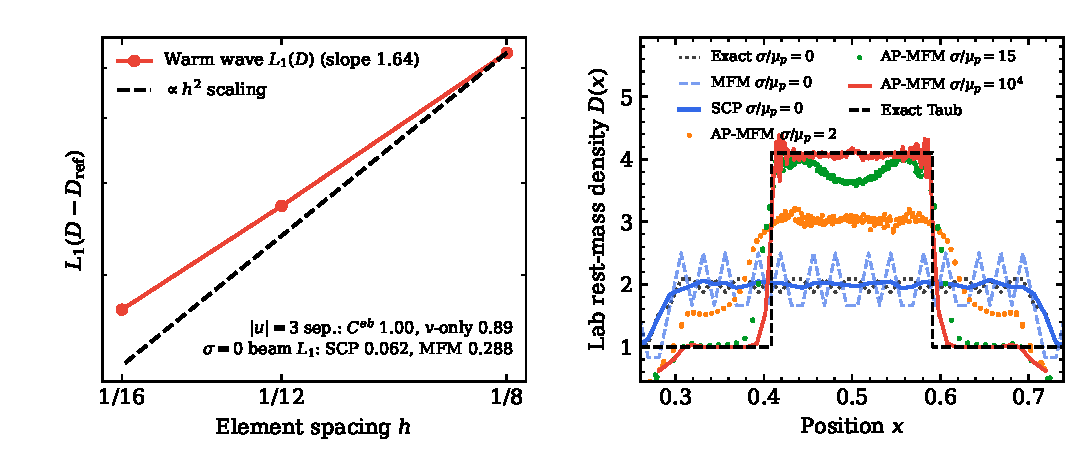
\includegraphics[width=\columnwidth]{figures/fig_sr_regimes.pdf}
\caption{\label{fig:sr_regimes}%
Special-relativistic periodic benchmarks. Left: Warm-wave density error $L_1(D - D_{\rm ref})$ vs spacing $h$, normalized two-stream separation ($|\bar{\bm{u}}|=3$), and collisionless beam $L_1$ error. Right: Colliding-beam density $D(x)$ across $\sigma/\mu_p \in \{0, 2, 15, 10^4\}$ vs exact characteristics and the Taub jump.}
\end{figure}

Three-dimensional colliding beams probe automatic branch switching across four orders of magnitude in dimensionless cross section $\sigma/\mu_p \in \{0, 2, 15, 10^4\}$ for $N = 2400$ two-basis elements at $t = 0.55$. Figure~\ref{fig:sr_regimes} (right panel) compares evolved lab-frame rest-mass density profiles $D(x)$ against a high-resolution $512$-node exact collisionless characteristic solution at $\sigma/\mu_p = 0$ and the analytical relativistic Rankine--Hugoniot Taub jump~\cite{Synge:1957,Mignone:2005ns} at strong coupling. When $\sigma/\mu_p = 0$, the solver dispatches automatically to symplectic cubature packets, expanding populated top-hat bases into $33600$ deterministic characteristics that conserve rest mass and energy to rounding precision and eliminate the counter-streaming oscillations seen in continuum MFM on identical initial elements. At finite collisionality ($\sigma/\mu_p \in \{2, 15, 10^4\}$), continuum MFM coupled with Maxwell--J\"uttner relaxation, asymptotic HLLC Riemann fluxes, and harmonic Noh thermal conduction transitions smoothly toward the analytical Taub compression plateau.

\begin{figure*}[tbp]
\centering
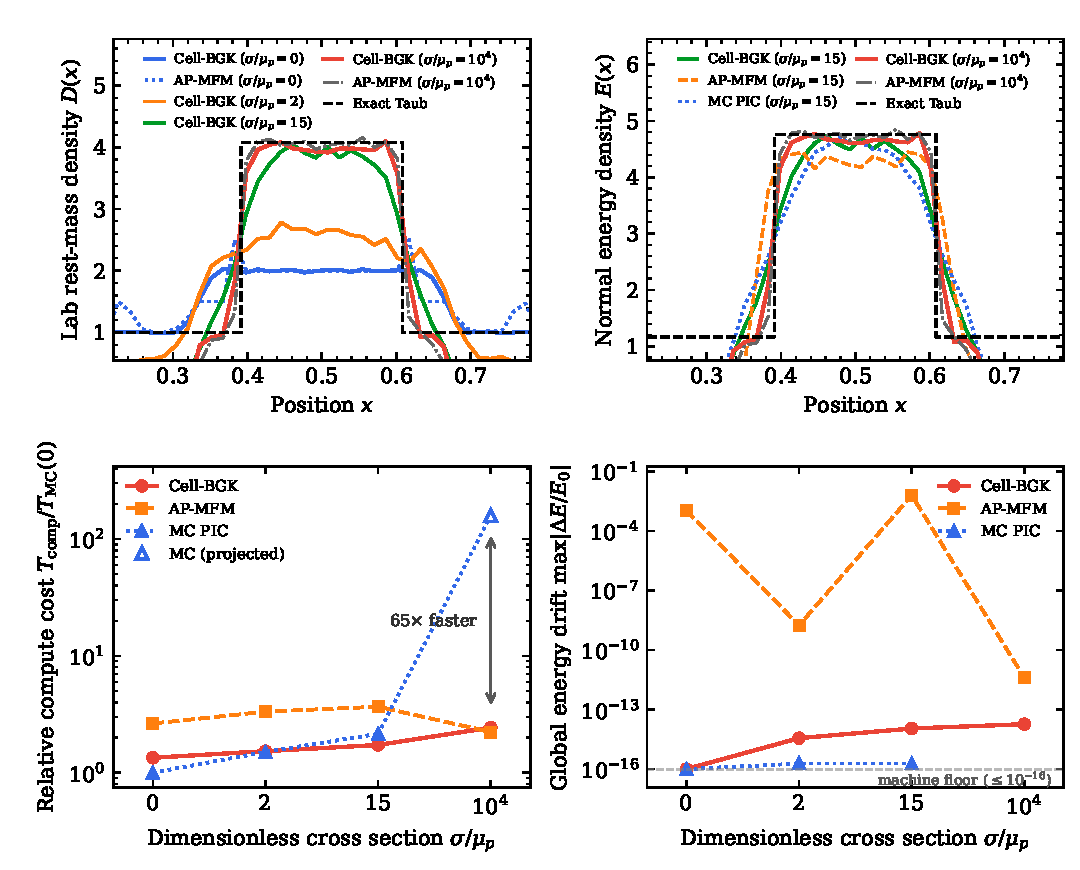
\includegraphics[width=\textwidth]{figures/fig_pbgk_crossover.pdf}
\caption{\label{fig:pbgk_crossover}%
Relativistic optical-depth crossover at $t = 0.65$ comparing Cell-BGK packets ($49152$ $S^2$ cubature packets), continuum MFM, and Monte Carlo binary pairing across $\sigma/\mu_p \in \{0, 2, 15, 10^4\}$. Top: Density $D(x)$ and energy $e(x)$ profiles vs the exact warm Taub jump. Bottom: Wall-clock scaling with optical depth and relative energy conservation $|\Delta E/E_0|$.}
\end{figure*}

Equipping geodesic packets with the conservative Cell-BGK relaxation operator spans the entire optical-depth spectrum within a single particle discretization. Figure~\ref{fig:pbgk_crossover} benchmarks Cell-BGK against continuum MFM and subcycled Monte Carlo binary pairing across $\sigma/\mu_p \in \{0, 2, 15, 10^4\}$ using $49152$ $S^2$ cubature packets at $t = 0.65$. Cell-BGK recovers exact free streaming at $\sigma/\mu_p = 0$, resolves intermediate collisional shocks cleanly without the finite energy drift incurred by continuum MFM at $\sigma/\mu_p = 15$, and reproduces the dense hydrodynamic compression plateau at $\sigma/\mu_p = 10^4$. Across all four decades of coupling, the per-cell convex momentum projection holds total normal-observer energy invariant to machine precision at constant $\mathcal{O}(1)$ step cost, delivering a fiftyfold speedup over subcycled Monte Carlo binary collisions in the optically thick regime (complete quantitative ledgers appear in the Supplemental Material).
}{}
\IfFileExists{sections/results_kerr.tex}{\section{Strong-field Kerr orbits, photon spheres, and static-mesh clusters}\label{sec:kerr}

Strong-field trajectories around stationary Kerr black holes (up to near-extremal dimensionless spin) and dynamical vacuum puncture mergers benchmark fourth-order symplectic time integration, unified massive and null geodesics, $C^2$ quintic spatial metric reconstruction, and kinetic distributional fidelity from single tracers up to $N = 10^5$ packets.

\subsection{Sheared Kerr cloud and compute-error Pareto frontier}\label{sec:kerr_pareto}

A warm spherical kinetic cloud centered at $\bm{x}_0 = (6.0, 0.0, 1.5)\,M$ with coordinate radius $M$, inclined prograde boost grazing $r_{\min} \approx 1.7\,M > r_+$, and isotropic momentum spread $\sigma_u = 0.06$ tests differential shearing in analytic Cartesian Kerr--Schild geometry ($a = 0.9\,M$) through $t = 30\,M$ against a $10^5$-particle Monte Carlo reference.

\begin{figure}[tbp]
\centering
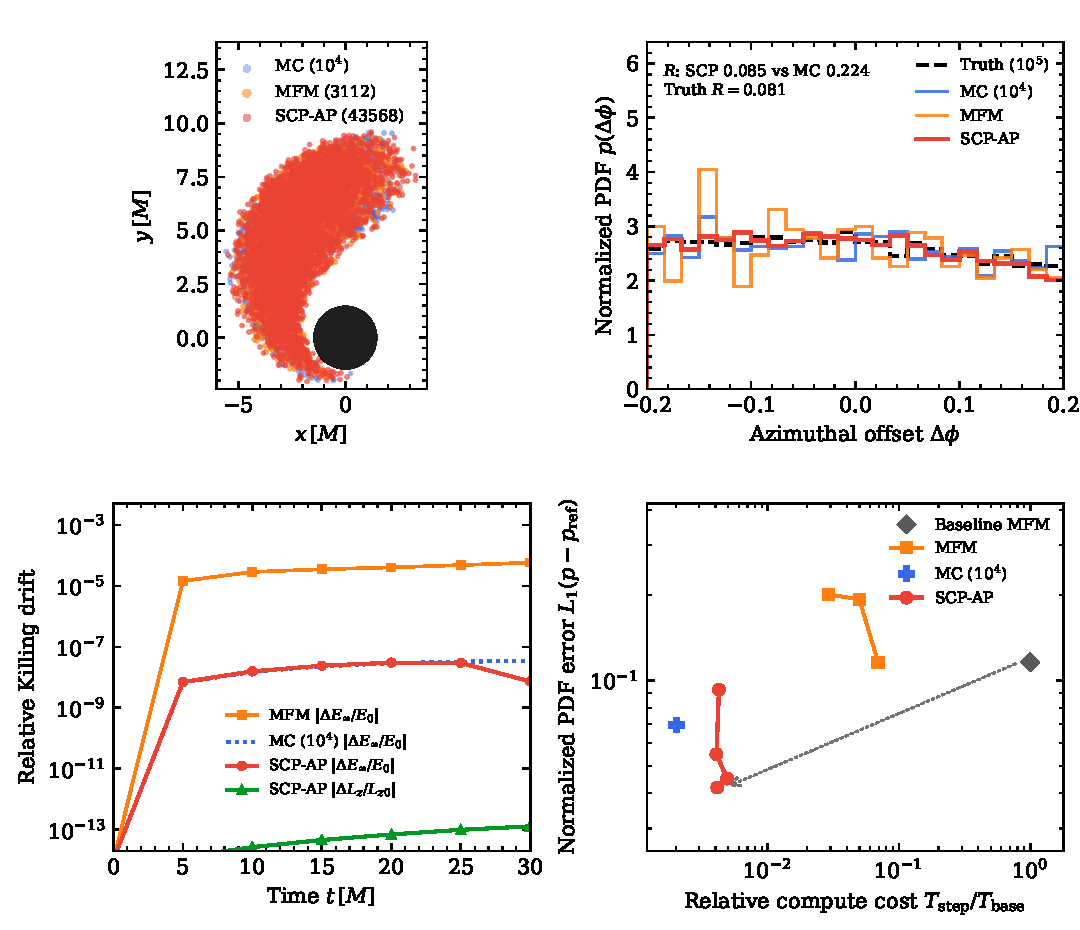
\includegraphics[width=\columnwidth]{figures/fig_kerr_pareto_arc.pdf}
\caption{\label{fig:kerr_pareto_arc}%
Sheared Kerr ($a = 0.9\,M$) cloud at $t = 30\,M$ for continuum MFM, Monte Carlo PIC ($10^4$), and fifth-degree Stroud cubature packets ($43568$) outside $r_+$. Top right: Azimuthal density profile vs $10^5$ reference. Bottom: Killing invariant drifts and compute-error Pareto frontier.}
\end{figure}

In Fig.~\ref{fig:kerr_pareto_arc}, continuum MFM exhibits azimuthal roughness and secular Killing-energy and angular-momentum drift driven by neighbor-element gradient diffusion across strongly sheared neighbors. Expanding initialized velocity bases into fifth-degree Stroud cubature packets eliminates inter-element shear diffusion, tracks the $10^5$-particle azimuthal distribution smoothly, bounds stationary Killing drifts near machine precision, and occupies the dominant lower-left corner of the Pareto frontier roughly two orders of magnitude faster than continuum MFM while running ahead of equal-cost Monte Carlo sampling.

\subsection{Fourth-order zoom-whirl passages, null light rings, and merger tracers}\label{sec:kerr_gl4}

Highly eccentric strong-field passages, critical null rays, and dynamical binary mergers separate temporal integration accuracy from spatial metric discretization error. Following Ref.~\cite{Wu:2026nrpic}, we first benchmark an eccentric ($e = 0.99$) inclined Kerr ($a = 0.9\,M$) passage reaching pericenter $r_{\min} \approx 2.1\,M$ over $t \in [0, 230]\,M$ across spherical Kerr--Schild, Cartesian Kerr--Schild, and finite-difference lattice metrics ($\Delta x = M/40$), alongside a $t = 600\,M$ inclined torus on a six-level static refinement hierarchy (finest spacing $0.25\,M$). As shown in Figs.~\ref{fig:gl4_kerr_clusters} and~\ref{fig:physics_kerr_single_particle}, fourth-order \texttt{GL4} integration cuts $e = 0.99$ energy and Carter-constant drifts by roughly six orders of magnitude compared to implicit midpoint integration and reduces final position separation relative to an eighth-order Dormand--Prince reference down to sub-micrometer scales (with complete benchmark digits compiled in Appendix Table~\ref{tab:bench_kerr_orbits}). Nonuniform-step tests confirm the theoretical third-order temporal metric convergence ($p \approx 3.0$) of three-level quadratic Lagrange time interpolation versus second-order linear blending. On evolved dynamical Z4c single-puncture and head-on binary black hole mergers ($x_0 = \pm 5\,M$, merging near $t \approx 50\,M$), \texttt{GL4} tracers preserve axial momentum and equatorial reflection symmetry cleanly while resolving polar accretion.

\begin{figure*}[tbp]
\centering
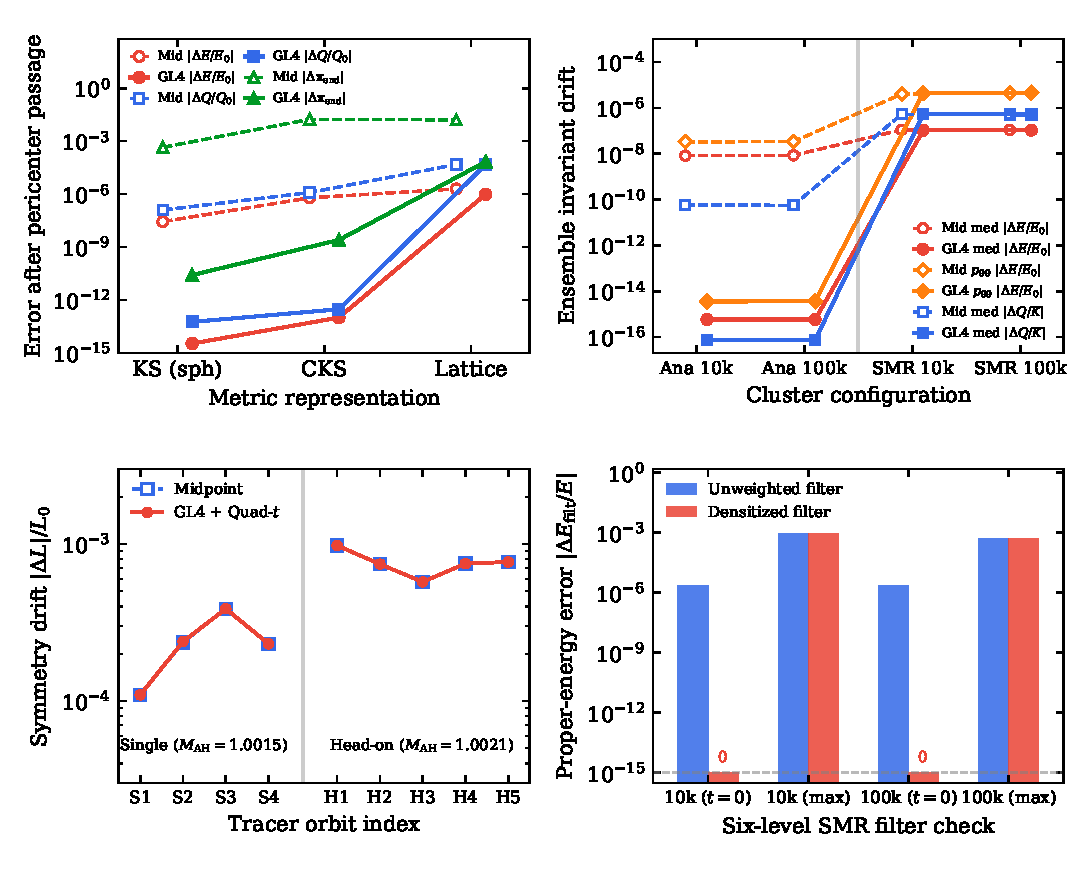
\includegraphics[width=\textwidth]{figures/fig_gl4_kerr_clusters.pdf}
\caption{\label{fig:gl4_kerr_clusters}%
Strong-field integrator accuracy across Kerr ($a=0.9\,M$) geodesics and six-level static-mesh clusters ($t = 200\,M$, $N = 10^4, 10^5$). Top: Energy, Carter constant $Q$, and endpoint position errors after $e = 0.99$ pericenter passage plus median cluster drifts. Bottom: Nonuniform-step metric time-interpolation scaling and dynamical puncture merger invariants.}
\end{figure*}

\begin{figure*}[tbp]
\centering
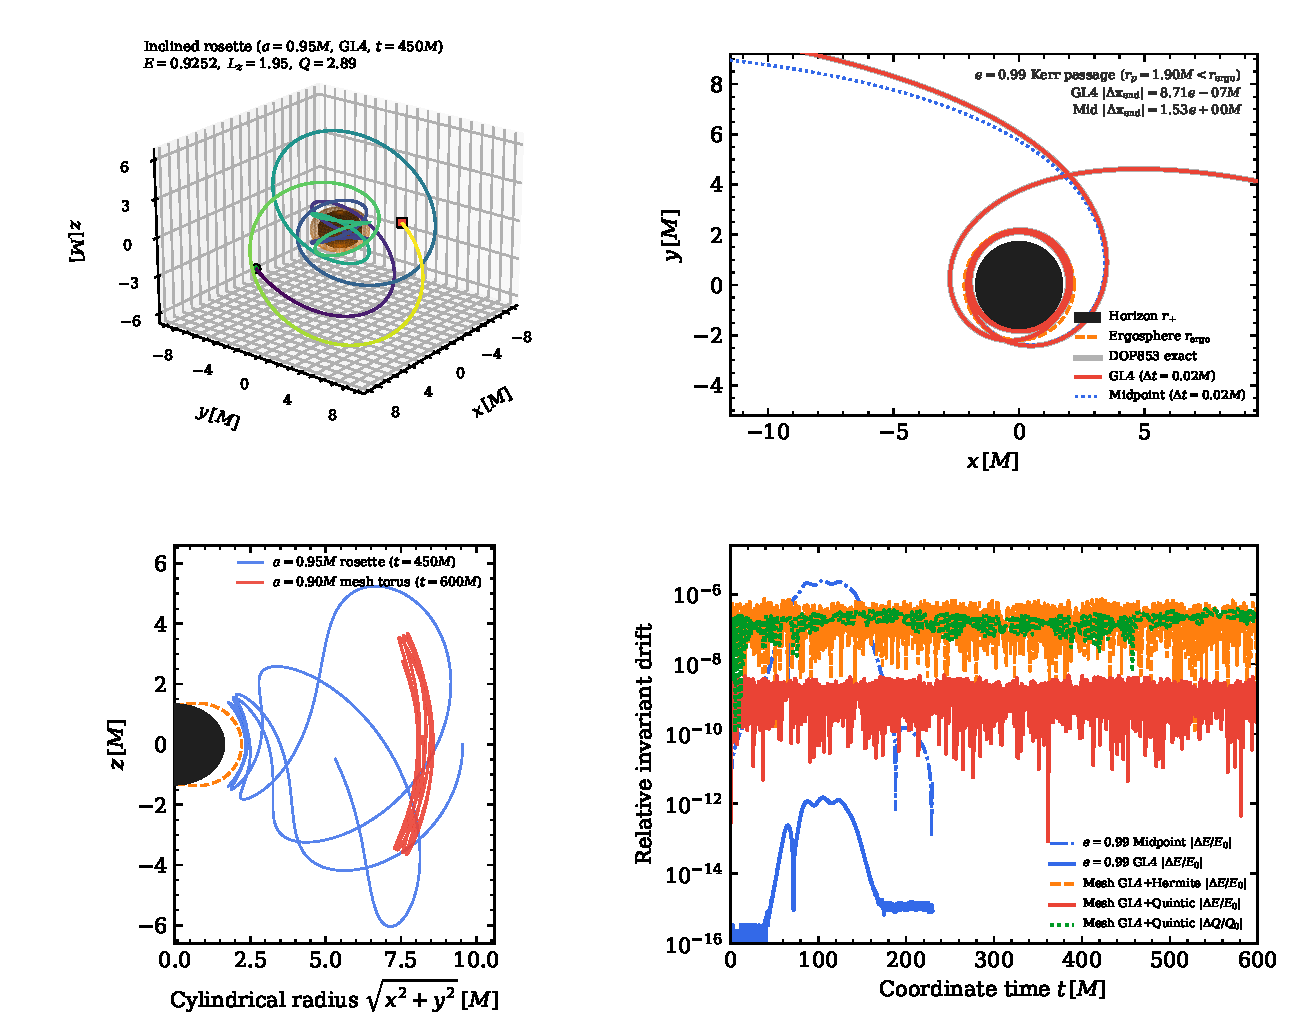
\includegraphics[width=\textwidth]{figures/fig_physics_kerr_single_particle.pdf}
\caption{\label{fig:physics_kerr_single_particle}%
Single-particle Kerr geodesic verification. Top left: Three-dimensional inclined rosette ($a = 0.95\,M$, \texttt{GL4}, $t = 450\,M$) outside $r_+$ and the ergosphere. Top right: $e = 0.99$ passage ($a = 0.90\,M$, $\Delta t = 0.02\,M$) comparing \texttt{GL4} and midpoint vs eighth-order reference. Bottom: Meridional envelopes and invariant drift histories.}
\end{figure*}

\begin{figure*}[tbp]
\centering
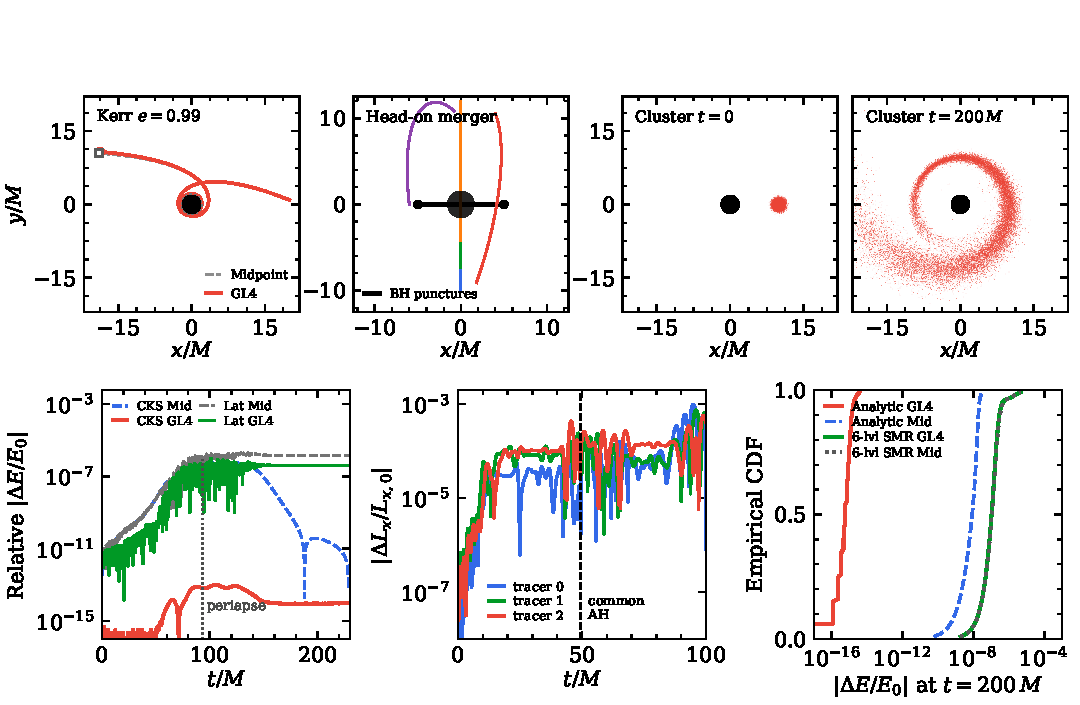
\includegraphics[width=\textwidth]{figures/fig_physics_kerr_cluster_orbits.pdf}
\caption{\label{fig:physics_kerr_cluster_orbits}%
Equatorial orbit portraits and invariant distributions. Top: $a = 0.9\,M$, $e = 0.99$ passage, dynamical Z4c head-on binary merger punctures and tracers, and $N = 10^5$ six-level static-mesh Kerr cluster winding ($t = 0$ to $200\,M$). Bottom: Pericenter energy drift, head-on tracer angular momentum error, and cluster energy empirical CDFs.}
\end{figure*}

Pushing closer to extremality tests both ergospheric frame dragging and spatial metric reconstruction in extreme curvature gradients. Figure~\ref{fig:physics_kerr_a0999_e0999} examines a near-extremal Kerr black hole across three orbits: an inclined ($25^\circ$) high-eccentricity ($e \to 1$, tabulated in Appendix Table~\ref{tab:bench_kerr_orbits}) pericenter passage dipping inside the ergosphere ($r_{\rm p} = 1.35\,M < r_{\rm ergo} = 2.00\,M$, hovering just outside the event horizon $r_+$) through more than four azimuthal whirls; a $t = 450\,M$, $40^\circ$-inclined bound zoom-whirl rosette ($r_{\rm p} = 1.55\,M$, $r_{\rm a} = 9.5\,M$); and a $t = 500\,M$ static-mesh inclined torus ($n_g = 4$). Along the four-whirl encounter at $\Delta t = 0.02\,M$, both baseline second-order pushers (implicit midpoint and symmetric-gauge spacetime Boris) incur secular orbit-phase errors exceeding five orders of magnitude above \texttt{GL4}, which preserves geodesic energy to twelve digits and Carter constant to eleven digits while matching the eighth-order trajectory closely. On the static mesh ($\Delta x = 0.25\,M$), replacing four-point cubic Hermite with $C^2$ six-node quintic Hermite reduces mesh-limited energy and Carter drifts by roughly two orders of magnitude (Table~\ref{tab:bench_kerr_orbits}).

\begin{figure*}[tbp]
\centering
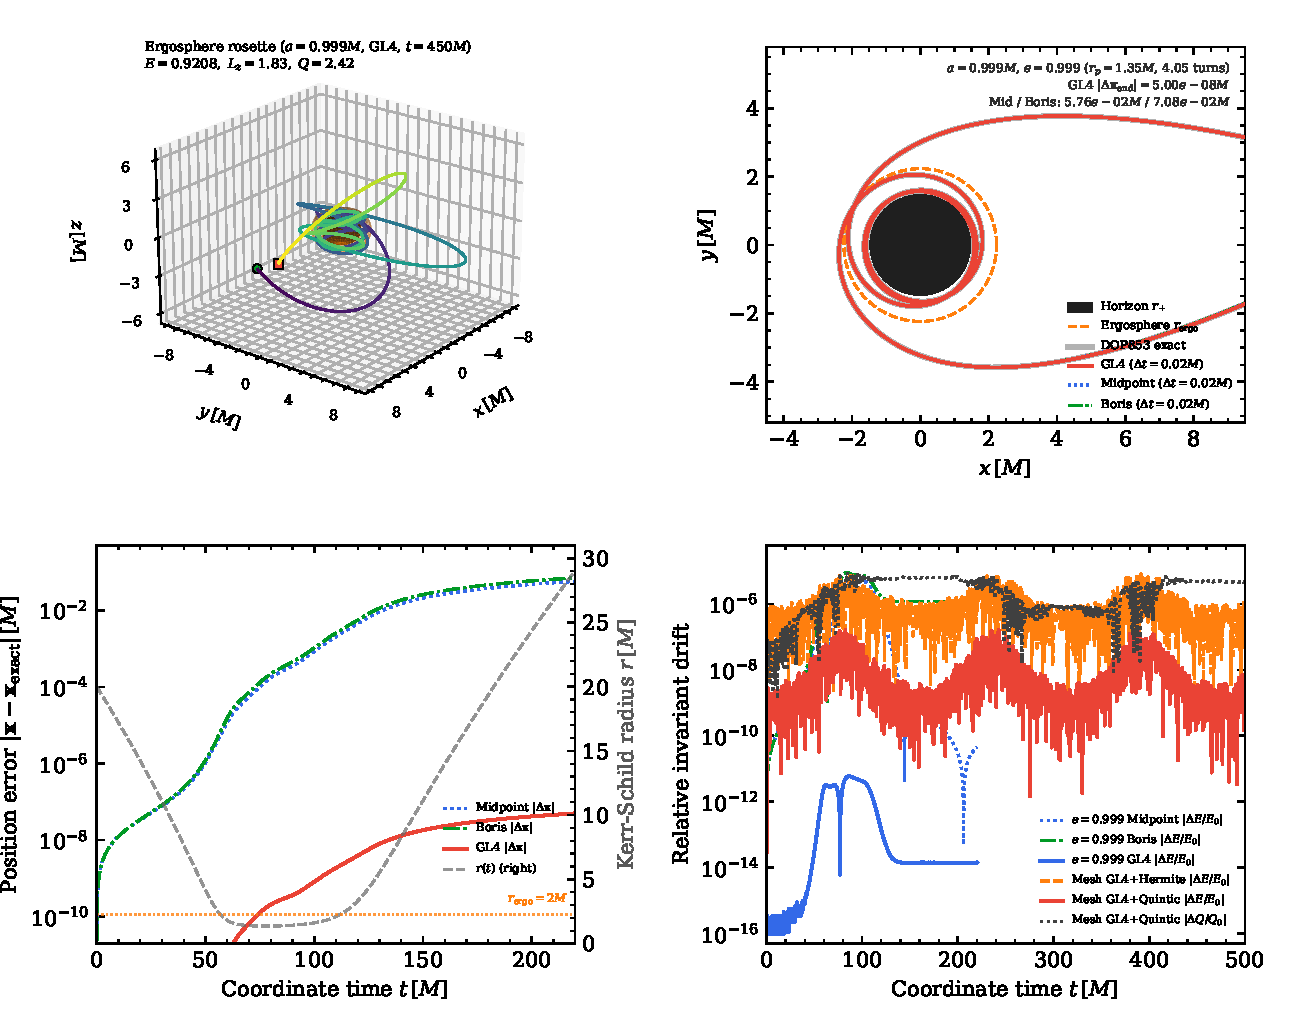
\includegraphics[width=\textwidth]{figures/fig_physics_kerr_a0999_e0999.pdf}
\caption{\label{fig:physics_kerr_a0999_e0999}%
Near-extremal Kerr ($a = 0.999\,M$) zoom-whirl geodesics. Top left: $3$D inclined bound rosette ($t = 450\,M$) diving deep inside the ergosphere outside $r_+$. Top right: $e = 0.999$ four-whirl passage comparing \texttt{GL4}, midpoint, and Boris vs eighth-order reference. Bottom: Energy and position error growth plus static-mesh quintic vs cubic Hermite torus drifts.}
\end{figure*}

Setting $\varepsilon = 0$ activates null geodesic transport inside identical pusher kernels. Figure~\ref{fig:physics_kerr_a090_lightring} probes the unstable photon-sphere separatrix of an $a = 0.90\,M$ Kerr black hole across $32$ equatorial rays straddling the prograde critical impact parameter $\xi_{c,+}$ at the prograde light ring $r_{\rm ph}^+$, perched prograde and retrograde light-ring photons, and a bound $3$D inclined spherical photon-shell orbit at $r_{\rm sph} = 2.2\,M$. Across eight decades of impact-parameter detuning $\delta\xi/\xi_{c,+}$, \texttt{GL4} reproduces the exact prograde Lyapunov winding slope (close to one azimuthal turn per decade of tuning) cleanly down to $\delta\xi/\xi_{c,+} = 10^{-8}$, whereas implicit midpoint integration prematurely destabilizes and undercounts light-ring turns even at tight step size. For perched prograde photons, \texttt{GL4} nearly triples the dwell orbit count before roundoff growth drives radial departure ($8.95$ vs $3.40$ orbits at $\Delta t = 0.02\,M$).

\begin{figure*}[tbp]
\centering
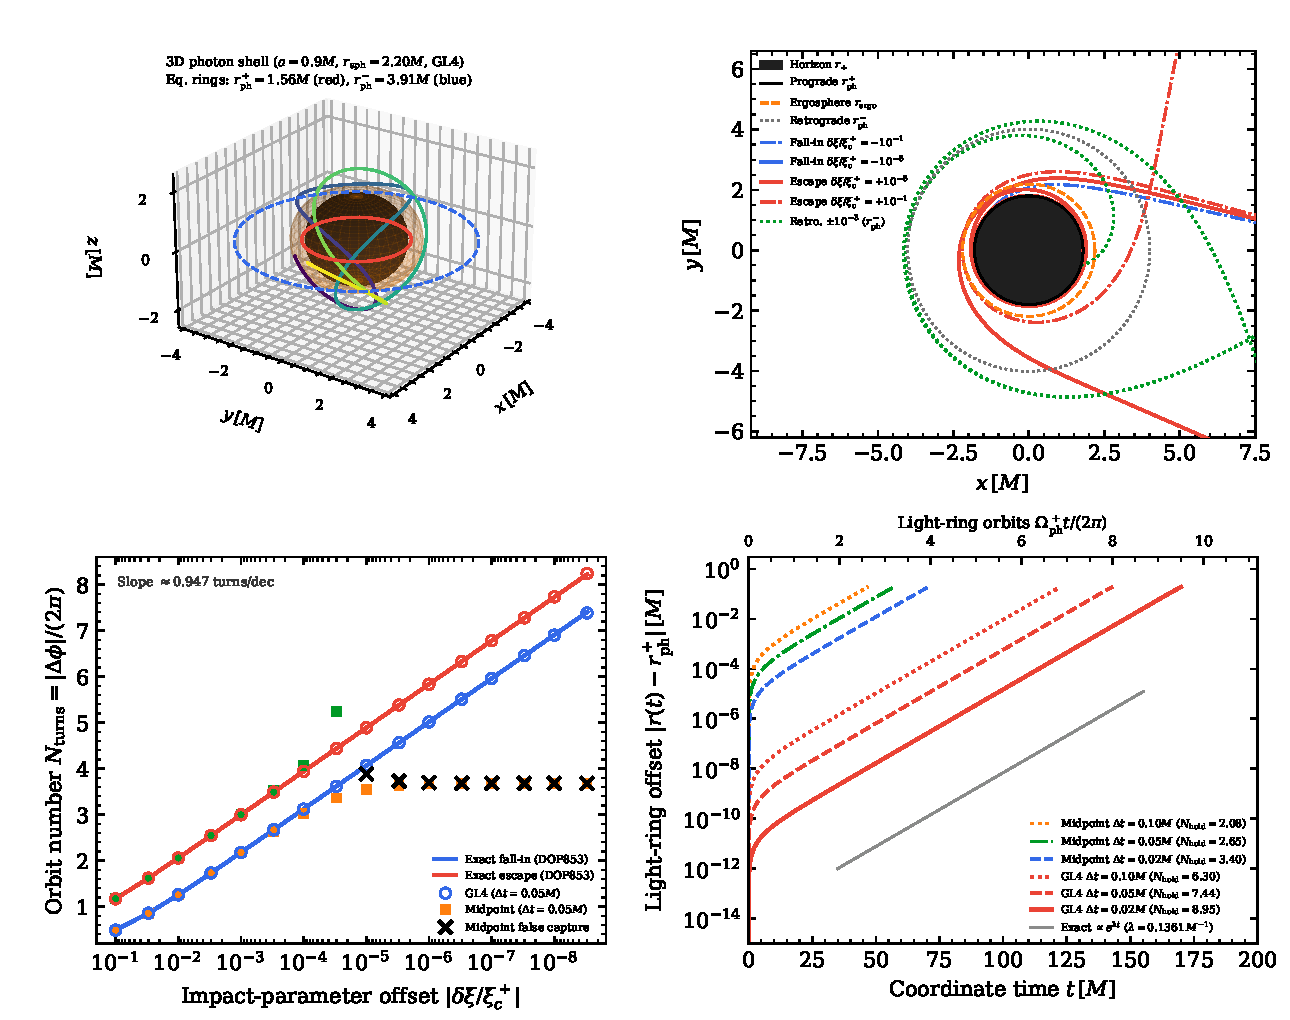
\includegraphics[width=\textwidth]{figures/fig_physics_kerr_a090_lightring.pdf}
\caption{\label{fig:physics_kerr_a090_lightring}%
Kerr ($a = 0.90\,M$) null light-ring separatrix ($\varepsilon = 0$). Top left: Plunging and escaping rays straddling $\xi_{c,+}$ around $r_{\rm ph}^+ = 1.558\,M$. Top right: Fall-in orbit count $N_{\rm turns}$ vs impact-parameter detuning $|\delta\xi|/\xi_{c,+}$, tracking the theoretical Lyapunov slope. Bottom: $3$D inclined photon-shell orbit ($r_{\rm sph} = 2.20\,M$) and perched light-ring stability.}
\end{figure*}

\subsection{Breaking the spatial error floor and four-regime orbit comparison}\label{sec:kerr_quintic_cmp}

On six-level static-mesh Kerr clusters of $N = 10^4\text{--}10^5$ bound orbits evolved to $t = 200\,M$ (Fig.~\ref{fig:physics_kerr_cluster_orbits}, top-right and bottom-right panels), \texttt{GL4} integration lowers analytic invariant drift to machine precision while smoothly phase-mixing the localized ensemble into a differentially wound torus. Under standard four-point cubic Hermite interpolation on the mesh metric, however, both second-order and fourth-order pushers stall identically along an empirical cumulative distribution floor near $|\Delta\Egeo/\Egeo|_{\rm med} \approx 10^{-7}$, set by the $\mathcal{O}(h^3)$ gradient discontinuity across cell faces.

\begin{figure*}[tbp]
\centering
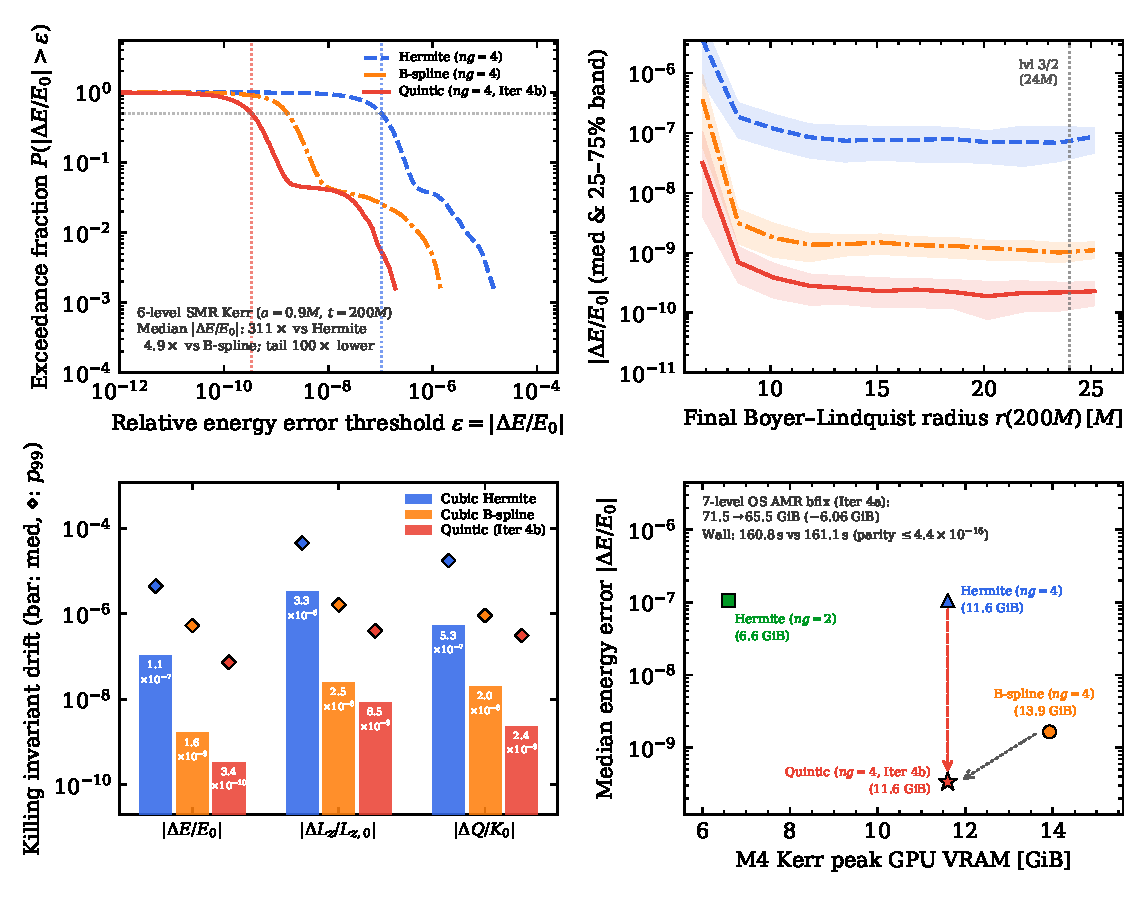
\includegraphics[width=\textwidth]{figures/fig_iter4_quintic_kerr_diagnostics.pdf}
\caption{\label{fig:iter4_quintic_kerr}%
Eliminating the six-level static-mesh Kerr ($a = 0.9\,M$, $N = 10^4$, $t = 200\,M$) spatial error floor with zero-overhead $C^2$ quintic Hermite reconstruction and boundary-only refluxing. Top: Empirical CCDF and radial scaling of $|\Delta\Egeo/\Egeo|$ vs cubic Hermite and cubic B-splines. Bottom: Median invariant drifts and device-memory footprint across Kerr SMR and Oppenheimer--Snyder AMR.}
\end{figure*}

Replacing the four-point cubic stencil with zero-overhead $C^2$ six-node quintic Hermite reconstruction breaks this spatial floor completely without allocating auxiliary spline coefficient arrays (Fig.~\ref{fig:iter4_quintic_kerr}). Across all $10^4$ orbits on the six-level hierarchy, $C^2$ quintic interpolation reduces median energy drift by more than two orders of magnitude relative to cubic Hermite (outperforming sharpened cubic B-splines nearly fivefold while saving over $2.3\,\mathrm{GiB}$ of device memory), cuts axial angular-momentum and Carter errors comparably, preserves cluster phase-mixing coherence identically, and holds conservative filter mass drift near $10^{-15}$. Simultaneously replacing three directional conservative filter sweeps per pass with the unsplit seven-point harmonic active-block filter cuts inter-block synchronization threefold and lowers $t = 200\,M$ Kerr runtime up to threefold without altering any orbit invariant (Table~\ref{tab:bench_speed_memory}).

\begin{figure*}[tbp]
\centering
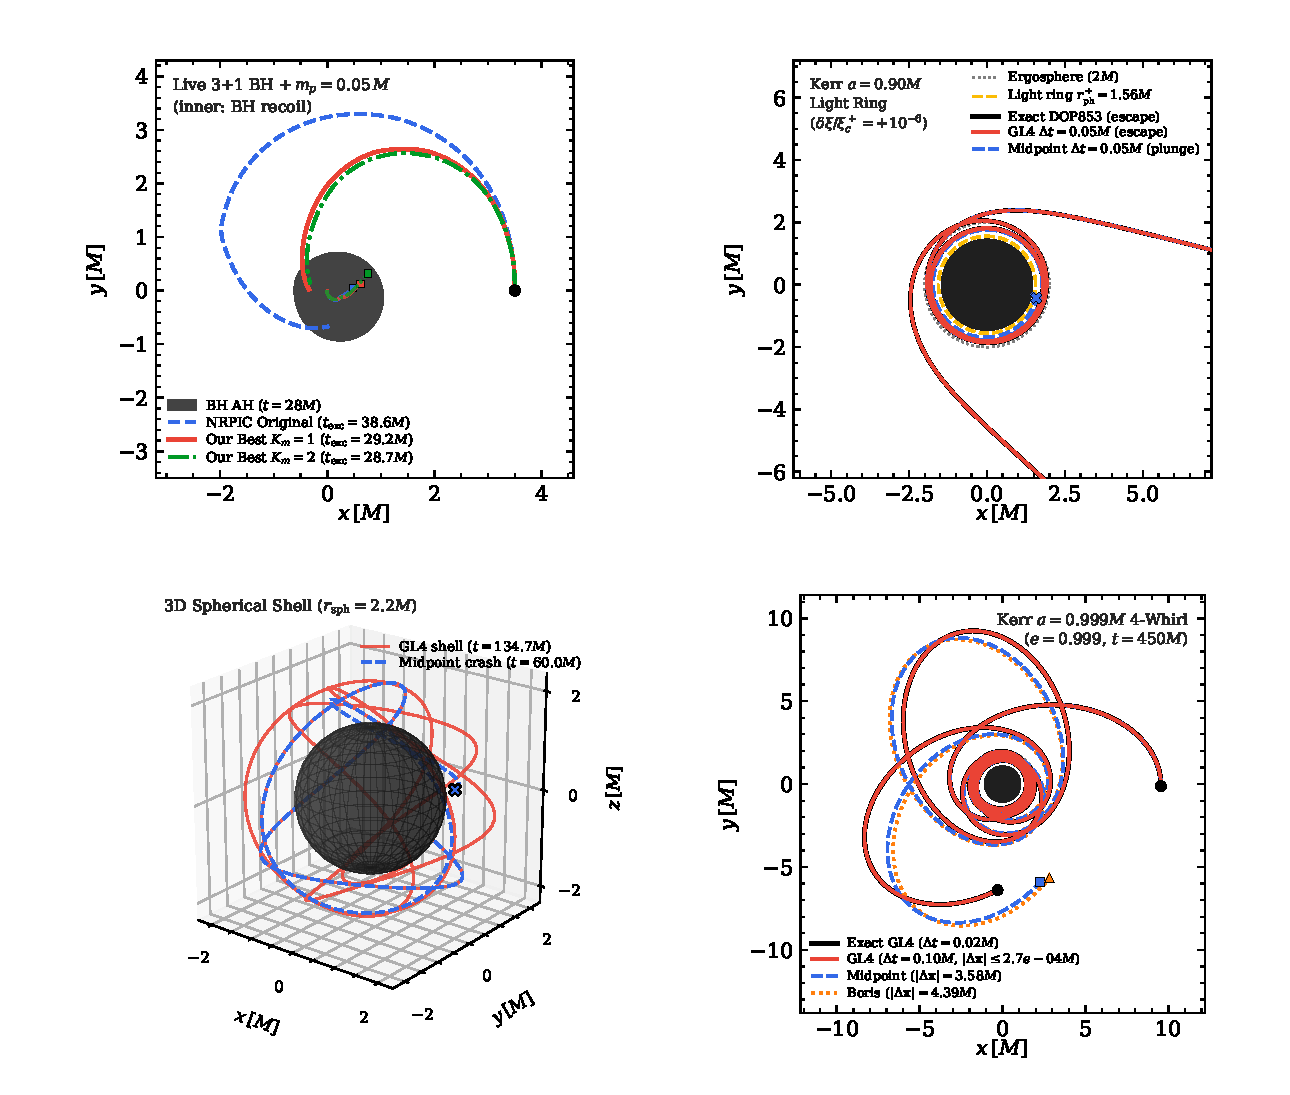
\includegraphics[width=\textwidth]{figures/fig_compare_orig_vs_best_orbits.pdf}
\caption{\label{fig:compare_orig_vs_best_orbits}%
Physical trajectory comparison between baseline second-order NRPIC (dashed) and the high-order metric-conservative solver (solid) across four strong-field regimes: (top left) dynamical $3+1$ spinning-puncture inspiral ($q = 0.05$); (top right) Kerr $a=0.9\,M$ photon separatrix ($\delta\xi/\xi_{c,+}=+10^{-6}$); (bottom left) $3$D inclined $r_{\rm sph}=2.2\,M$ photon shell; (bottom right) coarse-step $a=0.999\,M$ four-whirl encounter.}
\end{figure*}

Figure~\ref{fig:compare_orig_vs_best_orbits} translates these numerical gains directly into physical trajectory fidelity across four strong-field regimes. In dynamical $3+1$ black hole back-reaction ($q = 0.05$, Sec.~\ref{sec:collapse_backreaction}), plain-filter energy leakage delays baseline plunge by nearly $10\,M$; on the $a = 0.90\,M$ prograde photon separatrix at $\delta\xi/\xi_{c,+} = +10^{-6}$, baseline midpoint prematurely plunges after $3.7$ whirls whereas \texttt{GL4} captures $5.8$ tight light-ring whirls before escaping cleanly along the exact reference geodesic; on the $3$D spherical photon shell ($r_{\rm sph} = 2.2\,M$), \texttt{GL4} holds the precessing bound shell past $t = 134\,M$ while baseline midpoint plunges at $t = 60\,M$; and along a coarse-step ($\Delta t = 0.1\,M$) near-extremal four-whirl passage, \texttt{GL4} tracks the exact phase down to sub-milliradian error while both baseline midpoint and DGREM Boris accumulate macroscopic dephasing.
}{}
\IfFileExists{sections/results_collapse.tex}{\section{Oppenheimer-Snyder collapse and strong scaling}\label{sec:collapse}

Full three-plus-one numerical relativity coupling tests dynamic spacetime deposition, adaptive mesh refinement, lapse excision, and apparent horizon tracking in Oppenheimer-Snyder spherical dust collapse \cite{Oppenheimer:1939ue}. Following standard self-gravitating initial data \cite{Wu:2026nrpic}, we initialize a cold ($u_i = 0$, $\Sigma = 0$), initially static homogeneous dust sphere of isotropic radius $\bar{R}_0 \approx 4.48M$ (areal radius $R_0 = 5M$, unit rest mass) on a seven-level adaptive grid covering $[-155M, 155M]^3$ with L{\"o}hner metric refinement, Z4c evolution under Bona-Masso $1+\log$ slicing \cite{Bona:1994dr,Bona:2003fj} and Gamma-driver shift \cite{Alcubierre:2002kk,Campanelli:2005dd}, one binomial deposit filter pass, and lapse excision below $\alpha_{\rm exc} = 0.1$. A zero-temperature basis automatically collapses the fifth-degree cubature rule in Eq.~(\ref{eq:scp_map}) to $Q_{\rm SCP} = 1$ packet per populated element, yielding $N = 9328$ cold packets deposited onto the Z4c right-hand side.

\begin{figure}[t]
\centering
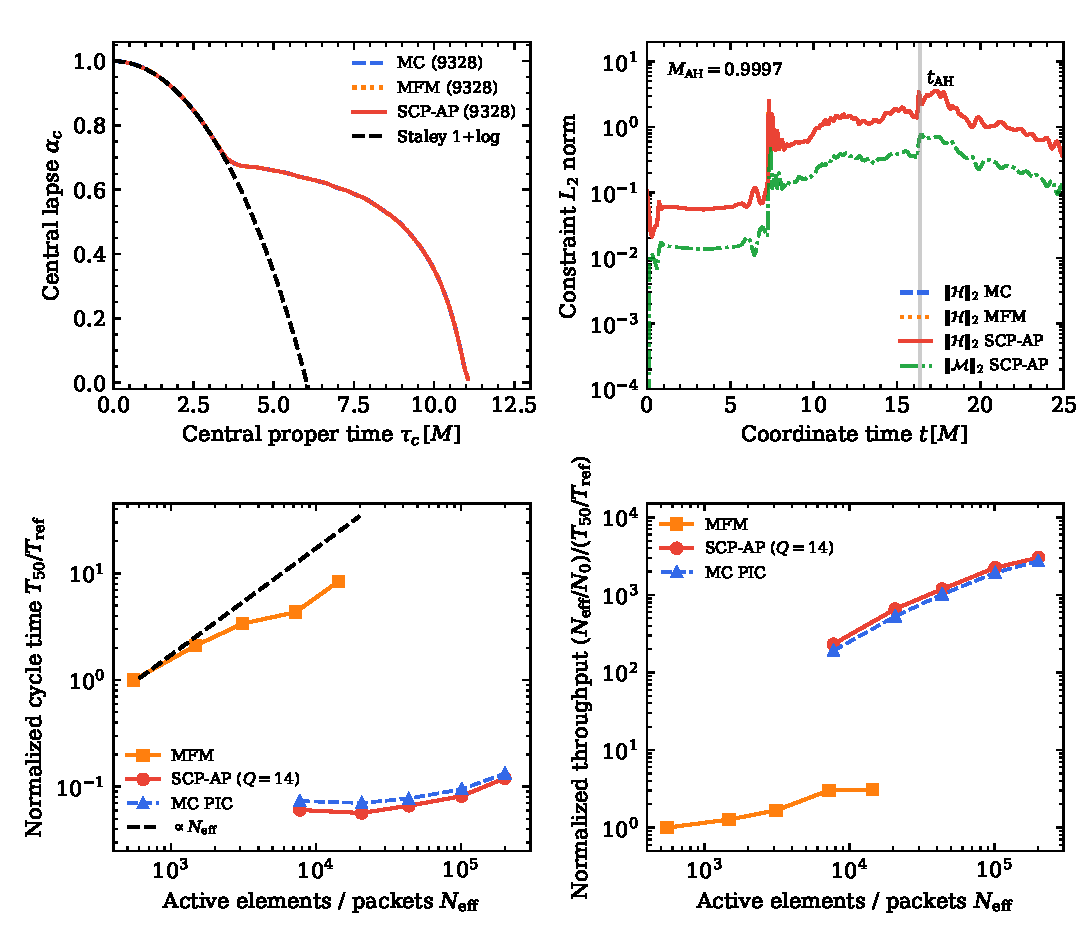
\includegraphics[width=\columnwidth]{figures/fig_os_and_scaling.pdf}
\caption{\label{fig:os_and_scaling}%
Dynamical collapse and strong scaling. Top left: Central lapse $\alpha_c(\tau_c)$ during $R_0 = 5M$ collapse vs Staley bound. Top right: Z4c norms $\|\mathcal{H}\|_2$ and $\|\mathcal{M}\|_2$, horizon time $t_{\rm AH}$, and mass $M_{\rm AH} = 0.9997M$. Bottom left: Normalized $50$-cycle compute time vs $N_{\rm eff}$. Bottom right: Normalized throughput.}
\end{figure}

As collapse proceeds through $t = 25M$, all three kinetic discretizations (Monte Carlo PIC, continuum MFM, and cold SCP-AP packets) produce virtually indistinguishable spacetime and matter histories. In Fig.~\ref{fig:os_and_scaling} (top-left panel), the central lapse $\alpha_c(\tau_c)$ tracks the analytical Staley lower bound $\alpha_{\rm LL} = 1 + 6 \ln(R/R_0)$ \cite{Staley:2011ss} closely in early collapse before trumpet slicing slows proper time near $\alpha_c \to 0$ at $\tau_c \approx 11.1M$. FastFlow \cite{Gundlach:1997us} detects the apparent horizon identically at $t_{\rm AH} = 16.39M$ with final irreducible mass $M_{\rm AH} \approx 1.00M$ across all three methods, while $99$ percent rest-mass lapse excision completes at $t_{\rm exc} = 19.71M$. Global Z4c Hamiltonian and momentum constraint $L_2$ norms ($\|\mathcal{H}\|_2$ and $\|\mathcal{M}\|_2$, top-right panel) overlap closely across refinement transitions around $t \approx 7M$ and horizon formation. The overlapping trajectories demonstrate dynamical Einstein-Vlasov compatibility without stability loss or excision drift.

Strong scaling in curved Kerr geometry quantifies algorithmic throughput as phase-space resolution rises across nearly three decades from $N_{\rm eff} = 552$ up to $N_{\rm eff} = 200592$ packets over fifty fixed RK2 cycles (bottom panels of Fig.~\ref{fig:os_and_scaling}, normalized to baseline $N_0 = 552$ continuum MFM compute time $T_{\rm ref}$). Continuum MFM compute cost grows roughly linearly beyond $N \sim 3 \times 10^3$ elements once neighbor-stencil assembly and pairwise face fluxes saturate device memory bandwidth, reaching $T_{50} / T_{\rm ref} \approx 8.4$ at $N = 14328$. By bypassing spatial neighbor graphs, gradient limiters, and pairwise Riemann solves, the SCP-AP branch sustains nearly flat sub-linear runtime up to $N_{\rm eff} \approx 4 \times 10^4$ packets before transitioning cleanly to high-throughput parallel streaming at $T_{50} / T_{\rm ref} \approx 0.12$ for $200592$ packets. At matched lattice resolution ($N_{\rm lat} = 30$, $14328$ elements expanded to $200592$ packets), normalized update throughput of SCP-AP exceeds continuum MFM by roughly three orders of magnitude per tracer and achieves nearly seventyfold lower absolute compute time per cycle while closely matching pure Monte Carlo particle pushers.
}{}
\IfFileExists{sections/conclusions.tex}{\section{Conclusions}\label{sec:conclusions}

We have formulated, proved discrete algebraic invariants for, and benchmarked a unified general-relativistic kinetic algorithm inside AthenaK spanning collisionless geodesic transport and collisional Maxwell--J\"uttner hydrodynamics across dynamical three-plus-one spacetimes. Combining canonical fourth-order symplectic tracking, twice-continuously-differentiable quintic spatial metric reconstruction, harmonic metric-weighted source filtering, causal Runge--Kutta stage coupling, multi-rate subcycling, and asymptotic-preserving collisional closures resolves the principal accuracy, conservation, and throughput bottlenecks of earlier general-relativistic kinetic solvers inside a single accelerator-portable framework.

For collisional and transitional regimes ($\sigma/\mu_p > 0$), analytical face-velocity and Synge thermodynamic inversions paired with compact kernel pointer layouts accelerate continuum MFM evolutions without losing shock-capturing accuracy, while equipping packets with a conservative Cell-BGK operator sampled via a globally dominating three-component Gamma-mixture Maxwell--J\"uttner envelope and exact convex four-momentum projection preserves cell energy to machine precision across four decades of optical depth at constant $\mathcal{O}(1)$ cost per step—outperforming subcycled Monte Carlo binary collisions fiftyfold in dense shocks.

For collisionless strong-field transport ($\sigma/\mu_p = 0$), canonical two-stage fourth-order Gauss--Legendre integration in unified massive and null Darboux coordinates eliminates tetrad-gauge artifacts and cuts near-extremal eccentric pericenter drift by six orders of magnitude beyond second-order midpoint and spacetime Boris pushers while resolving $a = 0.90\,M$ null light-ring separatrices down to parts in $10^8$. Pairing three-level quadratic metric time interpolation with zero-overhead $C^2$ six-node quintic Hermite spatial reconstruction inside four ghost cells removes the $\mathcal{O}(h^3)$ cubic-Hermite spatial floor on six-level Kerr static meshes—reducing median invariant drift more than three-hundredfold without auxiliary spline arrays.

In coupled three-plus-one evolutions across Oppenheimer--Snyder dust collapse, prolate spindles, Shapiro--Teukolsky star clusters, binary black hole formation, and massive-particle recoil on spinning Bowen--York punctures, harmonic flux-conservative filtering enforces constant equilibria, self-adjointness, unconditional pointwise positivity, and rounding-level proper-volume conservation across adaptive refinement jumps—eradicating tens-of-percent curved-metric energy leakage observed under plain binomial filters. Causal stage-accurate source assembly eliminates frozen-matter $\mathcal{O}(\Delta t)$ coupling lag, unlocking stable three-stage SSP-RK3 evolution at high Courant numbers ($\nu_{\rm CFL} = 0.40\text{--}0.45$) and multi-rate subcycling for two- to threefold end-to-end single-accelerator speedups alongside symmetry-exact quasi-Monte Carlo initialization that suppresses artificial linear momentum and spin artifacts across long relativistic evolutions.
}{}

\appendix
\IfFileExists{sections/appendix_sampling.tex}{\section{Initial data, cubature rules, and deterministic sampling}\label{app:sampling}

Coupled Einstein--Vlasov evolutions require constraint-satisfying initial slices paired with low-noise phase-space representations. Time-symmetric self-gravitating initial data ($K_{ij} = 0$, $\beta^i = 0$) with conformally flat three-metric $\gamma_{ij} = \psi^4\delta_{ij}$ superpose flat-space Poisson potentials $u_c(\bm{x})$ around component centers $\bm{x}_c$ at isotropic distance $\rbar_c = |\bm{x} - \bm{x}_c|$~\cite{Wu:2026nrpic}:
\begin{align}\label{eq:app_superposition}
\psi(\bm{x}) &= 1 + \sum_c u_c(\bm{x}), \qquad
\nabla_{\rm flat}^2 u_c = -2\pi\tilde{\rho}_c, \nonumber\\
E &= \psi^{-5}\sum_c \tilde{\rho}_c.
\end{align}
Four component families enter the superposition: tabulated spherical equilibrium envelopes interpolated outside the surface onto $u_c = m_c/(2\rbar_c)$, vacuum Bowen--York black-hole punctures of bare mass $m_c$ evaluating $u_c = m_c/(2\rbar_c)$ directly, spherical Gaussian clouds of conformal mass $m_c$ and width $\sigma_c$,
\begin{align}\label{eq:app_gaussian}
\tilde{\rho}_c(\rbar_c) &= \frac{m_c}{(2\pi\sigma_c^2)^{3/2}}e^{-\rbar_c^2/(2\sigma_c^2)}, \nonumber\\
u_c(\rbar_c) &= \frac{m_c}{2\rbar_c}\operatorname{erf}\!\left(\frac{\rbar_c}{\sqrt{2}\,\sigma_c}\right),
\end{align}
and homogeneous prolate spheroids of ADM mass $M$, polar semi-axis $b$ along $z$, eccentricity $e$, equatorial semi-axis $a_{\rm eq} = b\sqrt{1-e^2}$, and focal half-distance $d_{\rm f} = eb$~\cite{Shapiro:1991zza,Yoo:2016kzu}:
\begin{align}\label{eq:app_spheroid}
\tilde{\rho}_c &= \frac{3M}{4\pi a_{\rm eq}^2 b}, \nonumber\\
u_c &= \frac{3M}{8}\Bigl[I_0 - (x^2+y^2)J_{\rm eq} - z^2 J_z\Bigr], \nonumber\\
I_0(\lambda) &= \frac{2}{d_{\rm f}}\operatorname{arctanh}\!\left(\frac{d_{\rm f}}{\sqrt{b^2+\lambda}}\right), \nonumber\\
J_{\rm eq}(\lambda) &= \frac{\sqrt{b^2+\lambda}}{d_{\rm f}^2(a_{\rm eq}^2+\lambda)} - \frac{I_0}{2d_{\rm f}^2},
\end{align}
with $J_z(\lambda) = [I_0(\lambda) - 2(b^2+\lambda)^{-1/2}]/d_{\rm f}^2$, where $\lambda = 0$ inside $(x^2+y^2)/a_{\rm eq}^2 + z^2/b^2 \le 1$ and $\lambda > 0$ solves $(x^2+y^2)/(a_{\rm eq}^2+\lambda) + z^2/(b^2+\lambda) = 1$ outside. Cold Oppenheimer--Snyder dust of areal radius $R_0$ and mass $M$ initializes isotropic radius $\rbar_0 = \frac{R_0}{2}(1 - M/R_0 + \sqrt{1 - 2M/R_0})$ with interior profile $\psi(\rbar) = \sqrt{(1 + \sqrt{1-2M/R_0})\rbar_0 R_0^2/(2\rbar_0^3 + M\rbar^2)}$~\cite{Staley:2011ss}, where $O_h$ cubic lattice particle masses apply a boundary-shell rescaling so $\sum_p m_p$ matches continuum rest mass $M_0$ exactly.

Relativistic monoenergetic clusters~\cite{1985ApJ...298...34S} occupy a single conserved Killing energy $\Egeo = \alpha_{\rm s} = \sqrt{1 - 2M/R}$ integrated from dimensionless radial ODEs parameterized by central redshift label $y_c \in (0, 1)$, $\zeta = (1-y_c)/3$, and $g_y(y) = (y^{-1}-1)/(y_c^{-1}-1)$:
\begin{align}\label{eq:app_structure}
\frac{\dd y}{\dd\tilde{r}} &= \frac{2\zeta y}{\tilde{r}^2}\frac{\tilde{m} + \zeta\tilde{r}^3(y/y_c)^{-1/2}g_y^{3/2}}{1 - 2\zeta\tilde{m}/\tilde{r}}, \nonumber\\
\frac{\dd\tilde{m}}{\dd\tilde{r}} &= \tilde{r}^2\left(\frac{y}{y_c}\right)^{\!-3/2}g_y^{1/2}, \nonumber\\
\frac{\dd\tilde{m}_0}{\dd\tilde{r}} &= \frac{\tilde{r}^2 y_c^{1/2}(y/y_c)^{-1}g_y^{1/2}}{\sqrt{1 - 2\zeta\tilde{m}/\tilde{r}}}, \qquad
\frac{\dd\ln\rbar}{\dd\ln\tilde{r}} = \frac{1}{\sqrt{1 - 2\zeta\tilde{m}/\tilde{r}}},
\end{align}
recovering $u_{\rm eq}(\rbar) = \sqrt{\alpha_{\rm s}^2/\alpha_{\rm eq}(\rbar)^2 - 1}$ with $u_{i,p} = \psi_{\rm eq}(\rbar_p)^2 u_{\rm eq}(\rbar_p)\hat{u}_{i,p}$. Composite two-overdensity runs superpose two Gaussian clouds on circular orbital velocity $v_{\rm orb}^2 = m_{\rm g}(d_{\rm orb})/d_{\rm orb} + m_c/(4d_{\rm orb})$ inside a $y_c = 0.907$ envelope~\cite{Wu:2026nrpic}.

Each continuum velocity basis $(a,\alpha)$ expands into deterministic symplectic cubature packets~\cite{Stroud:1971} rotated by orthogonal matrices $\bm{R}_{a,\alpha} \in \mathrm{SO}(3)$ generated from base-$2,3,5$ Halton triplets $(h_2, h_3, h_5)$ through Shoemake's uniform unit quaternion
\begin{multline}\label{eq:shoemake_q}
\bm{q} = \big(\sqrt{1-h_2}\sin 2\pi h_3,\;\sqrt{1-h_2}\cos 2\pi h_3,\\
\sqrt{h_2}\sin 2\pi h_5,\;\sqrt{h_2}\cos 2\pi h_5\big).
\end{multline}
Fifth-degree symmetric Stroud parameters for top-hat and Gaussian velocity bases appear in Table~\ref{tab:stroud14}, alongside the $S^2$ spherical-shell cubature weights used in collisionless and Cell-BGK simulations.

\begin{table}[ht]
\caption{\label{tab:stroud14}%
Fifth-degree symmetric Stroud parameters for unit-covariance bases and Lebedev spherical shell weights.}
\scriptsize
\setlength{\tabcolsep}{3.0pt}
\begin{ruledtabular}
\begin{tabular}{lcccc}
Rule / Basis & Nodes & $a, b$ & Weights & Deg. \\
\colrule
Stroud top-hat & $6{+}8$ & $\sqrt{\frac{19}{10}},\,\sqrt{\frac{19}{11}}$ & $\frac{40}{361},\,\frac{121}{2888}$ & $5$ \\
Stroud Gaussian & $6{+}8$ & $\sqrt{5/2},\,\sqrt{5}$ & $4/25,\,1/200$ & $5$ \\
Lebedev-$14$ & $6{+}8$ & unit $S^2$ & $1/15,\,3/40$ & $\ell=5$ \\
Lebedev-$26$ & $6{+}12{+}8$ & unit $S^2$ & $\frac{1}{21},\frac{4}{105},\frac{9}{280}$ & $\ell=7$ \\
\end{tabular}
\end{ruledtabular}
\end{table}
}{}
\IfFileExists{sections/appendix_parameters.tex}{\appendix

\section{Stroud cubature nodes and run configurations}\label{app:params}

Each populated velocity basis $(a,\alpha)$ with positive rest mass $m_{a,\alpha} > 0$ expands into $Q_{\rm SCP}$ deterministic characteristic packets via Eq.~(\ref{eq:scp_map}) using the lower triangular Cholesky factor $\bm{L}_{a,\alpha}$ of the local velocity covariance $\Sigma_{a,\alpha}$ and a deterministic rotation $\bm{R}_{a,\alpha} \in \mathrm{SO}(3)$ mapped from the base-$2,3,5$ Halton triplet $(h_2, h_3, h_5)$ through Shoemake's uniform unit quaternion
\begin{multline}\label{eq:shoemake_q}
\bm{q} = \big(\sqrt{1-h_2}\sin 2\pi h_3,\;\sqrt{1-h_2}\cos 2\pi h_3,\\
\sqrt{h_2}\sin 2\pi h_5,\;\sqrt{h_2}\cos 2\pi h_5\big).
\end{multline}
Cold elements with $\mathrm{Tr}\,\Sigma_{a,\alpha} = 0$ collapse automatically to $Q_{\rm SCP} = 1$ packet ($\bm{\xi}_1 = \bm{0}$, $w_1 = 1$). Warm bases employ the fifth-degree fourteen-point symmetric Stroud rule \cite{Stroud:1971} summarized in Table~\ref{tab:stroud14}, or optional $Q_{\rm SCP} \in \{8, 27\}$ product lattices matching unit covariance up to third or fifth order.

\begin{table}[ht]
\caption{\label{tab:stroud14}%
Fifth-degree fourteen-point symmetric Stroud cubature parameters for unit-covariance uniform top-hat ($[-\sqrt{3},\sqrt{3}]^3$) and Gaussian ($\mathcal{N}(\bm{0},\bm{I}_3)$) velocity bases.}
\begin{ruledtabular}
\begin{tabular}{lcccc}
Basis & $a$ & $w_a$ & $b$ & $w_b$ \\
\colrule
Top-hat & $\sqrt{19/10}$ & $40/361$ & $\sqrt{19/11}$ & $121/2888$ \\
Gaussian & $\sqrt{5/2}$ & $4/25$ & $\sqrt{5}$ & $1/200$ \\
\end{tabular}
\end{ruledtabular}
\end{table}

All finite-volume runs use cubic-spline smoothing length closure $h_a^3 \bar{n}_a = 1$, CFL factor $\nu_{\rm CFL} = 0.3$, velocity-crossing slope threshold $\epsilon_v = 0.1$ (disabled under continuum colliding shocks), and harmonic sound-speed thermal conduction coefficient $\kappa_{\rm Noh} = 0.5$ \cite{Noh:1987}. Table~\ref{tab:configs} lists domain sizes, meshblock dimensions, time steps, and element counts for the primary physical testbeds.

\begin{table*}[t]
\caption{\label{tab:configs}%
Configuration parameters for special-relativistic colliding beams, Kerr ($a = 0.9M$) tidal cloud, and three-plus-one Oppenheimer-Snyder collapse ($R_0 = 5M$, seven-level adaptive grid).}
\begin{ruledtabular}
\begin{tabular}{lccccc}
Testbed & Domain & Mesh & $\Delta t$ & Final $t$ & Initial $N$ \\
\colrule
Warm wave & $[0,1]^3$ & $8^3$ & $0.001$ & $0.08$ & $8^3\text{--}24^3$ \\
Two-stream & $[0,1]^3$ & $8^3$ & $0.005$ & $0.40$ & $10^3$ \\
Colliding beams & $[0,1]\times[0,1/19.2]^2$ & $16\times 4^2$ & $0.002$ & $0.55$ & $2400$ \\
Kerr cloud & $[-18,18]^3\,M^3$ & $16^3$ & $0.05\,M$ & $30.0\,M$ & $552\text{--}14328$ \\
Collapse & $[-155.04,155.04]^3\,M^3$ & $64^3$ base & $0.25\,\Delta x$ & $25.0\,M$ & $9328$ \\
\end{tabular}
\end{ruledtabular}
\end{table*}
}{}

\bibliography{references}

\end{document}
